\section{Related Work}
\label{sec:related_work}

\begin{figure}[t]
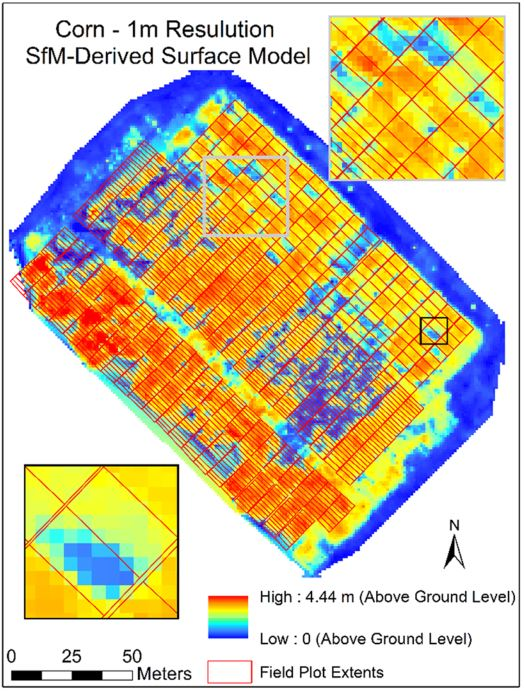
\includegraphics[width=\linewidth]{../images/DSM}
\caption{Digital surface models (DSMs). Adapted from \cite{UAV_HTPAR_2016}}
\label{fig:DSM}
\end{figure}

This work builds upon the research "Unmanned Aerial Vehicles for High-Throughput Phenotyping and Agronomic Research" \cite{UAV_HTPAR_2016}. In this study, the authors present four case studies involving multiple crops in breeding and agronomic applications developed by five teams: Administration, Flight Operations, Sensors, Data Management, and Field Research. As a pioneering project in its field, it provided valuable insights into critical sensor information, air vehicles, and configuration parameters for both. Using a UAV equipped with a high-resolution camera, images were collected from a large field of maize comprising 1,064 plots on July 22, 2015. A digital surface model (DSM) (Figure \ref{fig:DSM}) was calculated from the image data and employed to estimate plant height. These estimates were compared to ground truth measurements taken approximately three weeks earlier. The approach adopted in this study resulted in a correlation of ($r^2 = 0.35$; $p<0.0001$) for the first case study, where only 705 plots were analyzed as a group due to extensive feral hog damage sustained by a significant number of plots between the ground truth and imaging dates.

As per Shi \textit{et al.}\cite{UAV_HTPAR_2016}, the generally weak correlation between UAV estimates and ground truth plant height can be attributed to several factors:

The fixed-wing UAV estimates lacked sufficient resolution to distinguish the small tassels atop the plants, which were measured on the ground.

UAV images were collected approximately three weeks after ground truth data, and the plants had dried down significantly, resulting in a less erect plant canopy compared to earlier in the season.

Plot boundaries were manually drawn on the mosaicked image, introducing variability in pixel selection accuracy.

The bare ground DSM exhibited some elevation variation, which was not considered in UAV estimates of plant height.

Collectively, these issues suggest that process improvements are warranted and that future results are likely to be enhanced.

Similar published works utilize hyperspectral and multispectral imaging to accurately quantify field-scale phenotypic information and integrate the data into AI models \cite{jung2021potential} or provide growth monitoring methods using UAV data \cite{chang2017crop}.